\documentclass[12pt]{memoir}

\def\nsemestre {II}
\def\nterm {Fall}
\def\nyear {2024}
\def\nprofesor {Maria Gillespie}
\def\nsigla {MATH601}
\def\nsiglahead {Advanced Combinatorics}
\def\nextra {CHWA}
\def\nlang {ENG}
\input{../../headerVarillyDiff}
\usepackage{youngtab}

\begin{document}

\begin{Ej}
    Consider the dihedral group $D_4$ (the symmetry group of a square, including reflections and
rotations) acting on the plane by the corresponding reflection and rotation matrices. Show that this
representation of $D_4$ is an irreducible 2-dimensional representation over both $\bR$ and $\bC$.
\end{Ej}

\begin{ptcbr}
    Observe that we may present the dihedral group as 
$$\quot{\text{Free}(r,s)}{\gen(r^4,s^2,(sr)^2)}.$$
The desired representation is given by the action on the generators:
$$r\mapsto\twobytwo{0}{-1}{1}{0},\word{and}s\mapsto\twobytwo{1}{0}{0}{-1}.$$
Both matrices have $\vec{v}=\twobyone{1}{-1}$ as an eigenvector. This can be seen either by checking both eigenspaces or by looking at the row sums. Correspondingly, $r$ has eigenvalue $-1$ and $s$, a $1$.\par 
For both $\bR$ and $\bC$, the vector $\vec u=\twobyone{1}{1}$ lies in $\vec v^\perp$. To decompose our representation, we consider the basis $\cB=\set{\vec u,\vec v}$ along with the change of basis matrix 
$$M=\bonj{\id}_\cB^\cC=\twobytwo{1}{1}{1}{-1}\To M^{-1}=\bonj{\id}_\cC^\cB=\frac{1}{-2}\twobytwo{-1}{-1}{-1}{1}=\half M.$$
Conjugating our generators we obtain
\begin{align*}
\wt{r}=M^{-1}rM
&=\half\twobytwo{1}{1}{1}{-1}\twobytwo{0}{-1}{1}{0}\twobytwo{1}{1}{1}{-1}\\
&=\half\twobytwo{1}{1}{1}{-1}\twobytwo{-1}{1}{1}{1}\\
&=\half\twobytwo{0}{2}{-2}{0}\\
&=\half\twobytwo{0}{1}{-1}{0}
\end{align*}
and for the case of $s$:
\begin{align*}
    \wt{s}=M^{-1}sM
    &=\half\twobytwo{1}{1}{1}{-1}\twobytwo{1}{0}{0}{-1}\twobytwo{1}{1}{1}{-1}\\
    &=\half\twobytwo{1}{1}{1}{-1}\twobytwo{1}{1}{-1}{1}\\
    &=\half\twobytwo{0}{2}{2}{0}\\
    &=\half\twobytwo{0}{1}{1}{0}.
    \end{align*}

    So after conjugating, we can see that we cannot decompose the representation further. As indecomposability is equivalent to irreducibility in this case, we have that this representation is an irreducible 2-dimensional representation.
\end{ptcbr}

\begin{Ej}
    Prove that if $G$ is a finite abelian group, then all of its irreducible representations are 1-
dimensional. [Hint: you may want to look up some resources showing that commuting matrices are
simultaneously diagonalizable.]
\end{Ej}

\begin{ptcbr}
If $|G|=n$, then $g^n=\id_G$. If $\rho\:G\to\rGL(V)$ is our representation, then 
$$g^n=\id_G\To\rho(g)^n=I\To\rho(g)^n-I=0.$$
This means $\rho(g)$ satisfies the polynomial equation $z^n-1=0$. At first, this doesn't directly imply that $\rho(g)$ is diagonalizable, but with a careful eye we can remember about the minimal polynomial. The minimal polynomial of $\rho(g)$ divides any polynomial which annihilates $\rho(g)$ as it is the generator of the ideal of such polynomials:
$$\min_{\rho(g)}\mid z^n-1$$
and as $z^n-1$ splits into distinct linear factors, the minimal polynomial must be a product of such factors. Being the roots of $\min_{\rho(g)}$ all distinct, we have that $\rho(g)$ is diagonalizable.\par 
Now, as $G$ is abelian, we also have that the matrices $\set{\rho(g)\:\ g\in G}$ commute. Therefore they are all simultaneously diagonalizable.
\end{ptcbr}

\begin{Ej}
    Suppose $A$ is an $m\x m$ matrix and $B$ is an $n\x n$ matrix. Recall that the tensor product of the matrices $A$ and $B$ is the matrix having block form
    $$\nbyn{a_{11}B}{a_{12}B}{a_{1m}B}{a_{21}B}{a_{22}B}{a_{2m}B}{a_{m1}B}{a_{m2}B}{a_{mm}B}.$$
    Show that, if $\rho\: G\to\rGL(\bC^m)$ and $\sg\: G\to\rGL(\bC^n)$ are two representations of a group $G$ (thought of
as collections of matrices $\rho(g)$ and $\sg(g)$), then the tensor product of these two representations, defined
as the action of $G$ on $\bC^m\ox\bC^n$ by $g(v\ox w)=(gv)\ox(gw)$, is the map
$$\rho\ox\sg\: G\to\rGL(\bC^{mn})$$
given by 
$$(\rho\ox\sg)(g)=\rho(g)\ox\sg(g).$$
\end{Ej}

\begin{ptcbr}
    We must check that the new map does indeed define a representation. This means that:
    \begin{enumerate}
        \item Each element of $G$ is mapped to a matrix in $\rGL_{mn}$.
        \item The identity is precisely mapped to the identity matrix, and
        \item The map $\rho\ox\sg$ is a homomorphism.
    \end{enumerate}
    Firstly, if $g\in G$, call $\rho(g)=A$ and $\sg(g)=B$. Then 
    $$(\rho\ox\sg)(g)=\rho(g)\ox\sg(g)=A\ox B=\nbyn{a_{11}B}{a_{12}B}{a_{1m}B}{a_{21}B}{a_{22}B}{a_{2m}B}{a_{m1}B}{a_{m2}B}{a_{mm}B}$$
    which is a block matrix of $n^2$ blocks, all size $m\x m$. The resulting matrix indeed lives in $\rGL_{mn}$.\par
    For the second item, if $\id_G$ is our identity element, then $\rho(\id_G)=I_m$ and $\sg(\id_G)=I_n$. This means that 
    \begin{align*}
        (\rho\ox\sg)(\id_G)&=\rho(\id_G)\ox\sg(\id_G)\\
        &=I_m\ox I_n\\
        &=\nbyn{\dl_{11}I_n}{\dl_{12}I_n}{\dl_{1m}I_n}{\dl_{21}I_n}{\dl_{22}I_n}{\dl_{2m}I_n}{\dl_{m1}I_n}{\dl_{m2}I_n}{\dl_{mm}I_n}\\
        &=\nbyn{I_n}{0}{0}{0}{I_n}{0}{0}{0}{I_n}
    \end{align*}
    which is the $m\x m$ block matrix containing $I_n$ blocks through its diagonal. This is exactly $I_{mn}$.\par
    Finally call $C=\rho(h)$ and $D=\sg(h)$ for another $h\in G$. We wish to show that
    $$(\rho\ox\sg)(gh)=(\rho\ox\sg)(g)(\rho\ox\sg)(h).$$
    Expanding the definition on the left side we have 
    $$(\rho\ox\sg)(gh)=\rho(gh)\ox\sg(gh)=(\rho(g)\rho(h))\ox(\sg(g)\sg(h))=(AC)\ox(BD).$$
    Meanwhile on the right hand side we have 
    $$(\rho\ox\sg)(g)(\rho\ox\sg)(h)=(\rho(g)\ox\sg(g))(\rho(h)\ox\sg(h))=(A\ox B)(C\ox D).$$
    Comparing entries will show us that the result\footnote{This property is the mixed product property of the tensor product and matrix multiplication!} is indeed true: Observe that 
    $$(AC)_{ij}=\displaystyle\sum_{k=1}^{m}a_{ik}c_{kj}$$
    so that $(AC)\ox(BD)$ has block form: 
    $$\displaystyle\nbyn{\displaystyle\sum_{k=1}^{m}a_{1k}c_{k1}BD}{\displaystyle\sum_{k=1}^{m}a_{1k}c_{k2}BD}{\displaystyle\sum_{k=1}^{m}a_{1k}c_{km}BD}{\displaystyle\sum_{k=1}^{m}a_{2k}c_{k1}BD}{\displaystyle\sum_{k=1}^{m}a_{2k}c_{k2}BD}{\displaystyle\sum_{k=1}^{m}a_{2k}c_{km}BD}{\displaystyle\sum_{k=1}^{m}a_{mk}c_{k1}BD}{\displaystyle\sum_{k=1}^{m}a_{mk}c_{k2}BD}{\displaystyle\sum_{k=1}^{m}a_{mk}c_{km}BD}.$$
    But observe that we may rearrange the terms of an entry of this matrix as follows: 
    $$\sum_{k=1}^{m}a_{ik}c_{kj}BD=\sum_{k=1}^{m}(a_{ik}B)(c_{kj}D).$$
    This means that this sum computes the entry of the product of matrices whose entries are the blocks $a_{ij}B$ and $c_{ij}D$. But the matrices with those entries are precisely $A\ox B$ and $C\ox D$.\par
    After showing this three properties we have shown that the tensor product of representations is indeed a representation. 
\end{ptcbr}
\begin{Ej}
    Recall the RSK bijection from Math 502, and use an appropriate version of it to give a combinatorial proof that the dimensions of the spaces on both sides of the Schur-Weyl duality formula
    $$\bC^n\oxyox\bC^n=\bigoplus_\la V_\la\ox V^\la$$
    are equal. (Recall that the left hand side is a tensor product of k copies of $\bC^n$, and the right hand side
    is summing over all $\la$ of size $k$ with at most $n$ rows.)
    [Hint: You do not need to know the actual RSK algorithm to do this problem, only what objects it
    forms bijections between. This can be found in Stanley chapter 7, for instance.]
\end{Ej}

\begin{Ej}
    Use the $\eps$ method to find the Lie algebra associated to the Lie group $B_n\subseteq\rSL_n(\bC)$ of upper
triangular matrices in $\rSL_n(\bC)$.
\end{Ej}

\begin{ptcbr}
    First let us do a sanity check. It is not that easy for my to outirhgt believe that $B^{\rSL}_n$ is totally inside $B^{\rGL}_n$. Let's see why this is the case:\par
    In $\rGL_n$ we have the subgroups $\rSL_n$ and $B_n^{\rGL}$. It is true that $\rSL_n\cap B_n$ is nonempty, but we have determinant 1 matrices which are not triangular, and triangular matrices without determinant 1. Now let us assume that there are matrices in $B^{\rSL}_n$ not in $B^{\rGL}_n$. Such a matrix fixes the complete flag of $\bC^n$, but by virtue of being invertible, that matrix should be in $B^{\rGL}_n$. This means that 
    $$B^{\rSL}_n=B^{\rGL}_n\cap\rSL_n$$ 
    and so taking their Lie algebras we get 
    $$\lie{b}^{\gsl}_n=\lie{b}^{\lie{gl}}_n\cap\gsl_n$$
    which means that the Borel Lie subalgebra of $\gsl_n$ is the triangular matrices with zero trace.\par
    Knowing that the Borel subgroup inside $\rSL_n$ is the triangular matrices with determinant one, we may apply the $\eps$ method to arrive to 
    $$\det(I+\eps X)=1+\eps\tr(X)$$
    with the additional condition that $X$ is triangular. In the same fashion, we conclude that $\lie{b}^{\gsl}_n$ is the collection of triangular, traceless matrices.
\end{ptcbr}

\begin{Ej}
    Let $V_i$ be the irreducible representation of $\gsl_2(\bC)$ with highest weight $i$. Compute the
decomposition of $V_3\ox V_5$ into irreducibles.
\end{Ej}

\begin{ptcbr}
    We may use the L-diagram process to find the tensor product decomposition:
    \begin{center}
        

\tikzset{every picture/.style={line width=0.75pt}} %set default line width to 0.75pt        

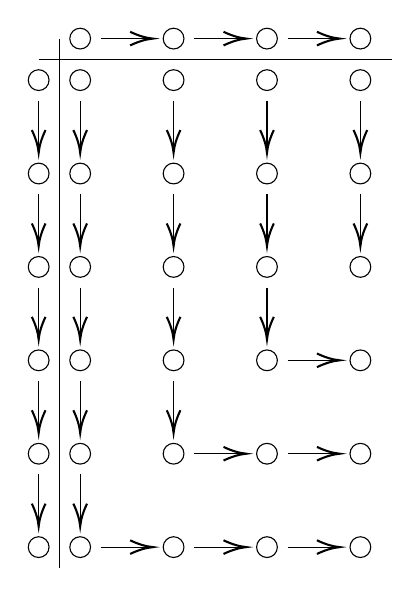
\begin{tikzpicture}[x=0.75pt,y=0.75pt,yscale=-1,xscale=1]
%uncomment if require: \path (0,300); %set diagram left start at 0, and has height of 300

%Shape: Circle [id:dp4977324245560253] 
\draw   (100,15) .. controls (100,12.24) and (102.24,10) .. (105,10) .. controls (107.76,10) and (110,12.24) .. (110,15) .. controls (110,17.76) and (107.76,20) .. (105,20) .. controls (102.24,20) and (100,17.76) .. (100,15) -- cycle ;
%Straight Lines [id:da526553918205122] 
\draw    (115,15) -- (138,15) ;
\draw [shift={(140,15)}, rotate = 180] [color={rgb, 255:red, 0; green, 0; blue, 0 }  ][line width=0.75]    (10.93,-3.29) .. controls (6.95,-1.4) and (3.31,-0.3) .. (0,0) .. controls (3.31,0.3) and (6.95,1.4) .. (10.93,3.29)   ;
%Shape: Circle [id:dp9010970930173063] 
\draw   (145,15) .. controls (145,12.24) and (147.24,10) .. (150,10) .. controls (152.76,10) and (155,12.24) .. (155,15) .. controls (155,17.76) and (152.76,20) .. (150,20) .. controls (147.24,20) and (145,17.76) .. (145,15) -- cycle ;
%Straight Lines [id:da8224303335477824] 
\draw    (160,15) -- (183,15) ;
\draw [shift={(185,15)}, rotate = 180] [color={rgb, 255:red, 0; green, 0; blue, 0 }  ][line width=0.75]    (10.93,-3.29) .. controls (6.95,-1.4) and (3.31,-0.3) .. (0,0) .. controls (3.31,0.3) and (6.95,1.4) .. (10.93,3.29)   ;
%Shape: Circle [id:dp7574431551679961] 
\draw   (190,15) .. controls (190,12.24) and (192.24,10) .. (195,10) .. controls (197.76,10) and (200,12.24) .. (200,15) .. controls (200,17.76) and (197.76,20) .. (195,20) .. controls (192.24,20) and (190,17.76) .. (190,15) -- cycle ;
%Straight Lines [id:da034619035756359384] 
\draw    (205,15) -- (228,15) ;
\draw [shift={(230,15)}, rotate = 180] [color={rgb, 255:red, 0; green, 0; blue, 0 }  ][line width=0.75]    (10.93,-3.29) .. controls (6.95,-1.4) and (3.31,-0.3) .. (0,0) .. controls (3.31,0.3) and (6.95,1.4) .. (10.93,3.29)   ;
%Shape: Circle [id:dp07092502681353607] 
\draw   (235,15) .. controls (235,12.24) and (237.24,10) .. (240,10) .. controls (242.76,10) and (245,12.24) .. (245,15) .. controls (245,17.76) and (242.76,20) .. (240,20) .. controls (237.24,20) and (235,17.76) .. (235,15) -- cycle ;
%Shape: Circle [id:dp6523825335476913] 
\draw   (84.95,30) .. controls (87.72,29.97) and (89.97,32.19) .. (90,34.95) .. controls (90.03,37.72) and (87.81,39.97) .. (85.05,40) .. controls (82.28,40.03) and (80.03,37.81) .. (80,35.05) .. controls (79.97,32.28) and (82.19,30.03) .. (84.95,30) -- cycle ;
%Straight Lines [id:da7948599829998227] 
\draw    (85,45) -- (85,68) ;
\draw [shift={(85,70)}, rotate = 270] [color={rgb, 255:red, 0; green, 0; blue, 0 }  ][line width=0.75]    (10.93,-3.29) .. controls (6.95,-1.4) and (3.31,-0.3) .. (0,0) .. controls (3.31,0.3) and (6.95,1.4) .. (10.93,3.29)   ;
%Shape: Circle [id:dp06342507122535068] 
\draw   (84.95,75) .. controls (87.72,74.97) and (89.97,77.19) .. (90,79.95) .. controls (90.03,82.72) and (87.81,84.97) .. (85.05,85) .. controls (82.28,85.03) and (80.03,82.81) .. (80,80.05) .. controls (79.97,77.28) and (82.19,75.03) .. (84.95,75) -- cycle ;
%Straight Lines [id:da3245441931269032] 
\draw    (85,90) -- (85,113) ;
\draw [shift={(85,115)}, rotate = 270] [color={rgb, 255:red, 0; green, 0; blue, 0 }  ][line width=0.75]    (10.93,-3.29) .. controls (6.95,-1.4) and (3.31,-0.3) .. (0,0) .. controls (3.31,0.3) and (6.95,1.4) .. (10.93,3.29)   ;
%Shape: Circle [id:dp2563432974496994] 
\draw   (84.95,120) .. controls (87.72,119.97) and (89.97,122.19) .. (90,124.95) .. controls (90.03,127.72) and (87.81,129.97) .. (85.05,130) .. controls (82.28,130.03) and (80.03,127.81) .. (80,125.05) .. controls (79.97,122.28) and (82.19,120.03) .. (84.95,120) -- cycle ;
%Straight Lines [id:da8557372863213878] 
\draw    (85,135) -- (85,158) ;
\draw [shift={(85,160)}, rotate = 270] [color={rgb, 255:red, 0; green, 0; blue, 0 }  ][line width=0.75]    (10.93,-3.29) .. controls (6.95,-1.4) and (3.31,-0.3) .. (0,0) .. controls (3.31,0.3) and (6.95,1.4) .. (10.93,3.29)   ;
%Shape: Circle [id:dp48564936421930427] 
\draw   (84.95,165) .. controls (87.72,164.97) and (89.97,167.19) .. (90,169.95) .. controls (90.03,172.72) and (87.81,174.97) .. (85.05,175) .. controls (82.28,175.03) and (80.03,172.81) .. (80,170.05) .. controls (79.97,167.28) and (82.19,165.03) .. (84.95,165) -- cycle ;
%Straight Lines [id:da039277984898681395] 
\draw    (85,180) -- (85,203) ;
\draw [shift={(85,205)}, rotate = 270] [color={rgb, 255:red, 0; green, 0; blue, 0 }  ][line width=0.75]    (10.93,-3.29) .. controls (6.95,-1.4) and (3.31,-0.3) .. (0,0) .. controls (3.31,0.3) and (6.95,1.4) .. (10.93,3.29)   ;
%Shape: Circle [id:dp44136244604923436] 
\draw   (84.95,210) .. controls (87.72,209.97) and (89.97,212.19) .. (90,214.95) .. controls (90.03,217.72) and (87.81,219.97) .. (85.05,220) .. controls (82.28,220.03) and (80.03,217.81) .. (80,215.05) .. controls (79.97,212.28) and (82.19,210.03) .. (84.95,210) -- cycle ;
%Straight Lines [id:da6794621957572885] 
\draw    (85,225) -- (85,248) ;
\draw [shift={(85,250)}, rotate = 270] [color={rgb, 255:red, 0; green, 0; blue, 0 }  ][line width=0.75]    (10.93,-3.29) .. controls (6.95,-1.4) and (3.31,-0.3) .. (0,0) .. controls (3.31,0.3) and (6.95,1.4) .. (10.93,3.29)   ;
%Shape: Circle [id:dp5126273860068598] 
\draw   (84.95,255) .. controls (87.72,254.97) and (89.97,257.19) .. (90,259.95) .. controls (90.03,262.72) and (87.81,264.97) .. (85.05,265) .. controls (82.28,265.03) and (80.03,262.81) .. (80,260.05) .. controls (79.97,257.28) and (82.19,255.03) .. (84.95,255) -- cycle ;
%Straight Lines [id:da4374129186438045] 
\draw    (85,25) -- (255,25) ;
%Straight Lines [id:da7544909366541875] 
\draw    (95,15) -- (95,270) ;
%Shape: Circle [id:dp15408865497892044] 
\draw   (104.95,30) .. controls (107.72,29.97) and (109.97,32.19) .. (110,34.95) .. controls (110.03,37.72) and (107.81,39.97) .. (105.05,40) .. controls (102.28,40.03) and (100.03,37.81) .. (100,35.05) .. controls (99.97,32.28) and (102.19,30.03) .. (104.95,30) -- cycle ;
%Straight Lines [id:da9602612804352613] 
\draw    (105,45) -- (105,68) ;
\draw [shift={(105,70)}, rotate = 270] [color={rgb, 255:red, 0; green, 0; blue, 0 }  ][line width=0.75]    (10.93,-3.29) .. controls (6.95,-1.4) and (3.31,-0.3) .. (0,0) .. controls (3.31,0.3) and (6.95,1.4) .. (10.93,3.29)   ;
%Shape: Circle [id:dp6142492628344308] 
\draw   (104.95,75) .. controls (107.72,74.97) and (109.97,77.19) .. (110,79.95) .. controls (110.03,82.72) and (107.81,84.97) .. (105.05,85) .. controls (102.28,85.03) and (100.03,82.81) .. (100,80.05) .. controls (99.97,77.28) and (102.19,75.03) .. (104.95,75) -- cycle ;
%Straight Lines [id:da9820429403510217] 
\draw    (105,90) -- (105,113) ;
\draw [shift={(105,115)}, rotate = 270] [color={rgb, 255:red, 0; green, 0; blue, 0 }  ][line width=0.75]    (10.93,-3.29) .. controls (6.95,-1.4) and (3.31,-0.3) .. (0,0) .. controls (3.31,0.3) and (6.95,1.4) .. (10.93,3.29)   ;
%Shape: Circle [id:dp7660260059604108] 
\draw   (104.95,120) .. controls (107.72,119.97) and (109.97,122.19) .. (110,124.95) .. controls (110.03,127.72) and (107.81,129.97) .. (105.05,130) .. controls (102.28,130.03) and (100.03,127.81) .. (100,125.05) .. controls (99.97,122.28) and (102.19,120.03) .. (104.95,120) -- cycle ;
%Straight Lines [id:da5774809152263051] 
\draw    (105,135) -- (105,158) ;
\draw [shift={(105,160)}, rotate = 270] [color={rgb, 255:red, 0; green, 0; blue, 0 }  ][line width=0.75]    (10.93,-3.29) .. controls (6.95,-1.4) and (3.31,-0.3) .. (0,0) .. controls (3.31,0.3) and (6.95,1.4) .. (10.93,3.29)   ;
%Shape: Circle [id:dp5972831185293573] 
\draw   (104.95,165) .. controls (107.72,164.97) and (109.97,167.19) .. (110,169.95) .. controls (110.03,172.72) and (107.81,174.97) .. (105.05,175) .. controls (102.28,175.03) and (100.03,172.81) .. (100,170.05) .. controls (99.97,167.28) and (102.19,165.03) .. (104.95,165) -- cycle ;
%Straight Lines [id:da11903735518654113] 
\draw    (105,180) -- (105,203) ;
\draw [shift={(105,205)}, rotate = 270] [color={rgb, 255:red, 0; green, 0; blue, 0 }  ][line width=0.75]    (10.93,-3.29) .. controls (6.95,-1.4) and (3.31,-0.3) .. (0,0) .. controls (3.31,0.3) and (6.95,1.4) .. (10.93,3.29)   ;
%Shape: Circle [id:dp7185989228085305] 
\draw   (104.95,210) .. controls (107.72,209.97) and (109.97,212.19) .. (110,214.95) .. controls (110.03,217.72) and (107.81,219.97) .. (105.05,220) .. controls (102.28,220.03) and (100.03,217.81) .. (100,215.05) .. controls (99.97,212.28) and (102.19,210.03) .. (104.95,210) -- cycle ;
%Straight Lines [id:da37084620231575405] 
\draw    (105,225) -- (105,248) ;
\draw [shift={(105,250)}, rotate = 270] [color={rgb, 255:red, 0; green, 0; blue, 0 }  ][line width=0.75]    (10.93,-3.29) .. controls (6.95,-1.4) and (3.31,-0.3) .. (0,0) .. controls (3.31,0.3) and (6.95,1.4) .. (10.93,3.29)   ;
%Shape: Circle [id:dp0723785227107423] 
\draw   (104.95,255) .. controls (107.72,254.97) and (109.97,257.19) .. (110,259.95) .. controls (110.03,262.72) and (107.81,264.97) .. (105.05,265) .. controls (102.28,265.03) and (100.03,262.81) .. (100,260.05) .. controls (99.97,257.28) and (102.19,255.03) .. (104.95,255) -- cycle ;
%Straight Lines [id:da41275476267279576] 
\draw    (115,260) -- (138,260) ;
\draw [shift={(140,260)}, rotate = 180] [color={rgb, 255:red, 0; green, 0; blue, 0 }  ][line width=0.75]    (10.93,-3.29) .. controls (6.95,-1.4) and (3.31,-0.3) .. (0,0) .. controls (3.31,0.3) and (6.95,1.4) .. (10.93,3.29)   ;
%Shape: Circle [id:dp17951240832110782] 
\draw   (145,260) .. controls (145,257.24) and (147.24,255) .. (150,255) .. controls (152.76,255) and (155,257.24) .. (155,260) .. controls (155,262.76) and (152.76,265) .. (150,265) .. controls (147.24,265) and (145,262.76) .. (145,260) -- cycle ;
%Straight Lines [id:da050172277423855216] 
\draw    (160,260) -- (183,260) ;
\draw [shift={(185,260)}, rotate = 180] [color={rgb, 255:red, 0; green, 0; blue, 0 }  ][line width=0.75]    (10.93,-3.29) .. controls (6.95,-1.4) and (3.31,-0.3) .. (0,0) .. controls (3.31,0.3) and (6.95,1.4) .. (10.93,3.29)   ;
%Shape: Circle [id:dp18272608669508228] 
\draw   (190,260) .. controls (190,257.24) and (192.24,255) .. (195,255) .. controls (197.76,255) and (200,257.24) .. (200,260) .. controls (200,262.76) and (197.76,265) .. (195,265) .. controls (192.24,265) and (190,262.76) .. (190,260) -- cycle ;
%Straight Lines [id:da9521193520549907] 
\draw    (205,260) -- (228,260) ;
\draw [shift={(230,260)}, rotate = 180] [color={rgb, 255:red, 0; green, 0; blue, 0 }  ][line width=0.75]    (10.93,-3.29) .. controls (6.95,-1.4) and (3.31,-0.3) .. (0,0) .. controls (3.31,0.3) and (6.95,1.4) .. (10.93,3.29)   ;
%Shape: Circle [id:dp2883479990166261] 
\draw   (235,260) .. controls (235,257.24) and (237.24,255) .. (240,255) .. controls (242.76,255) and (245,257.24) .. (245,260) .. controls (245,262.76) and (242.76,265) .. (240,265) .. controls (237.24,265) and (235,262.76) .. (235,260) -- cycle ;
%Shape: Circle [id:dp4670315060672986] 
\draw   (149.95,30) .. controls (152.72,29.97) and (154.97,32.19) .. (155,34.95) .. controls (155.03,37.72) and (152.81,39.97) .. (150.05,40) .. controls (147.28,40.03) and (145.03,37.81) .. (145,35.05) .. controls (144.97,32.28) and (147.19,30.03) .. (149.95,30) -- cycle ;
%Straight Lines [id:da44869803672113284] 
\draw    (150,45) -- (150,68) ;
\draw [shift={(150,70)}, rotate = 270] [color={rgb, 255:red, 0; green, 0; blue, 0 }  ][line width=0.75]    (10.93,-3.29) .. controls (6.95,-1.4) and (3.31,-0.3) .. (0,0) .. controls (3.31,0.3) and (6.95,1.4) .. (10.93,3.29)   ;
%Shape: Circle [id:dp4772095862094188] 
\draw   (149.95,75) .. controls (152.72,74.97) and (154.97,77.19) .. (155,79.95) .. controls (155.03,82.72) and (152.81,84.97) .. (150.05,85) .. controls (147.28,85.03) and (145.03,82.81) .. (145,80.05) .. controls (144.97,77.28) and (147.19,75.03) .. (149.95,75) -- cycle ;
%Straight Lines [id:da308090668576562] 
\draw    (150,90) -- (150,113) ;
\draw [shift={(150,115)}, rotate = 270] [color={rgb, 255:red, 0; green, 0; blue, 0 }  ][line width=0.75]    (10.93,-3.29) .. controls (6.95,-1.4) and (3.31,-0.3) .. (0,0) .. controls (3.31,0.3) and (6.95,1.4) .. (10.93,3.29)   ;
%Shape: Circle [id:dp36425505927230817] 
\draw   (149.95,120) .. controls (152.72,119.97) and (154.97,122.19) .. (155,124.95) .. controls (155.03,127.72) and (152.81,129.97) .. (150.05,130) .. controls (147.28,130.03) and (145.03,127.81) .. (145,125.05) .. controls (144.97,122.28) and (147.19,120.03) .. (149.95,120) -- cycle ;
%Straight Lines [id:da3846106037047944] 
\draw    (150,135) -- (150,158) ;
\draw [shift={(150,160)}, rotate = 270] [color={rgb, 255:red, 0; green, 0; blue, 0 }  ][line width=0.75]    (10.93,-3.29) .. controls (6.95,-1.4) and (3.31,-0.3) .. (0,0) .. controls (3.31,0.3) and (6.95,1.4) .. (10.93,3.29)   ;
%Shape: Circle [id:dp13194173735859271] 
\draw   (149.95,165) .. controls (152.72,164.97) and (154.97,167.19) .. (155,169.95) .. controls (155.03,172.72) and (152.81,174.97) .. (150.05,175) .. controls (147.28,175.03) and (145.03,172.81) .. (145,170.05) .. controls (144.97,167.28) and (147.19,165.03) .. (149.95,165) -- cycle ;
%Straight Lines [id:da9177956345072782] 
\draw    (150,180) -- (150,203) ;
\draw [shift={(150,205)}, rotate = 270] [color={rgb, 255:red, 0; green, 0; blue, 0 }  ][line width=0.75]    (10.93,-3.29) .. controls (6.95,-1.4) and (3.31,-0.3) .. (0,0) .. controls (3.31,0.3) and (6.95,1.4) .. (10.93,3.29)   ;
%Shape: Circle [id:dp5153931102350955] 
\draw   (149.95,210) .. controls (152.72,209.97) and (154.97,212.19) .. (155,214.95) .. controls (155.03,217.72) and (152.81,219.97) .. (150.05,220) .. controls (147.28,220.03) and (145.03,217.81) .. (145,215.05) .. controls (144.97,212.28) and (147.19,210.03) .. (149.95,210) -- cycle ;
%Straight Lines [id:da8936822812212525] 
\draw    (160,215) -- (183,215) ;
\draw [shift={(185,215)}, rotate = 180] [color={rgb, 255:red, 0; green, 0; blue, 0 }  ][line width=0.75]    (10.93,-3.29) .. controls (6.95,-1.4) and (3.31,-0.3) .. (0,0) .. controls (3.31,0.3) and (6.95,1.4) .. (10.93,3.29)   ;
%Shape: Circle [id:dp17972942292664118] 
\draw   (190,215) .. controls (190,212.24) and (192.24,210) .. (195,210) .. controls (197.76,210) and (200,212.24) .. (200,215) .. controls (200,217.76) and (197.76,220) .. (195,220) .. controls (192.24,220) and (190,217.76) .. (190,215) -- cycle ;
%Straight Lines [id:da6391572156024549] 
\draw    (205,215) -- (228,215) ;
\draw [shift={(230,215)}, rotate = 180] [color={rgb, 255:red, 0; green, 0; blue, 0 }  ][line width=0.75]    (10.93,-3.29) .. controls (6.95,-1.4) and (3.31,-0.3) .. (0,0) .. controls (3.31,0.3) and (6.95,1.4) .. (10.93,3.29)   ;
%Shape: Circle [id:dp04010851030649143] 
\draw   (235,215) .. controls (235,212.24) and (237.24,210) .. (240,210) .. controls (242.76,210) and (245,212.24) .. (245,215) .. controls (245,217.76) and (242.76,220) .. (240,220) .. controls (237.24,220) and (235,217.76) .. (235,215) -- cycle ;
%Shape: Circle [id:dp7681475038538963] 
\draw   (194.95,30) .. controls (197.72,29.97) and (199.97,32.19) .. (200,34.95) .. controls (200.03,37.72) and (197.81,39.97) .. (195.05,40) .. controls (192.28,40.03) and (190.03,37.81) .. (190,35.05) .. controls (189.97,32.28) and (192.19,30.03) .. (194.95,30) -- cycle ;
%Straight Lines [id:da08300795208380951] 
\draw    (195,45) -- (195,68) ;
\draw [shift={(195,70)}, rotate = 270] [color={rgb, 255:red, 0; green, 0; blue, 0 }  ][line width=0.75]    (10.93,-3.29) .. controls (6.95,-1.4) and (3.31,-0.3) .. (0,0) .. controls (3.31,0.3) and (6.95,1.4) .. (10.93,3.29)   ;
%Shape: Circle [id:dp2260771443817613] 
\draw   (194.95,75) .. controls (197.72,74.97) and (199.97,77.19) .. (200,79.95) .. controls (200.03,82.72) and (197.81,84.97) .. (195.05,85) .. controls (192.28,85.03) and (190.03,82.81) .. (190,80.05) .. controls (189.97,77.28) and (192.19,75.03) .. (194.95,75) -- cycle ;
%Straight Lines [id:da35361947959314344] 
\draw    (195,90) -- (195,113) ;
\draw [shift={(195,115)}, rotate = 270] [color={rgb, 255:red, 0; green, 0; blue, 0 }  ][line width=0.75]    (10.93,-3.29) .. controls (6.95,-1.4) and (3.31,-0.3) .. (0,0) .. controls (3.31,0.3) and (6.95,1.4) .. (10.93,3.29)   ;
%Shape: Circle [id:dp3352098686062388] 
\draw   (194.95,120) .. controls (197.72,119.97) and (199.97,122.19) .. (200,124.95) .. controls (200.03,127.72) and (197.81,129.97) .. (195.05,130) .. controls (192.28,130.03) and (190.03,127.81) .. (190,125.05) .. controls (189.97,122.28) and (192.19,120.03) .. (194.95,120) -- cycle ;
%Straight Lines [id:da8699467026582782] 
\draw    (195,135) -- (195,158) ;
\draw [shift={(195,160)}, rotate = 270] [color={rgb, 255:red, 0; green, 0; blue, 0 }  ][line width=0.75]    (10.93,-3.29) .. controls (6.95,-1.4) and (3.31,-0.3) .. (0,0) .. controls (3.31,0.3) and (6.95,1.4) .. (10.93,3.29)   ;
%Shape: Circle [id:dp35214676154591507] 
\draw   (194.95,165) .. controls (197.72,164.97) and (199.97,167.19) .. (200,169.95) .. controls (200.03,172.72) and (197.81,174.97) .. (195.05,175) .. controls (192.28,175.03) and (190.03,172.81) .. (190,170.05) .. controls (189.97,167.28) and (192.19,165.03) .. (194.95,165) -- cycle ;
%Straight Lines [id:da799113698224833] 
\draw    (205,170) -- (228,170) ;
\draw [shift={(230,170)}, rotate = 180] [color={rgb, 255:red, 0; green, 0; blue, 0 }  ][line width=0.75]    (10.93,-3.29) .. controls (6.95,-1.4) and (3.31,-0.3) .. (0,0) .. controls (3.31,0.3) and (6.95,1.4) .. (10.93,3.29)   ;
%Shape: Circle [id:dp8356853405689824] 
\draw   (235,170) .. controls (235,167.24) and (237.24,165) .. (240,165) .. controls (242.76,165) and (245,167.24) .. (245,170) .. controls (245,172.76) and (242.76,175) .. (240,175) .. controls (237.24,175) and (235,172.76) .. (235,170) -- cycle ;
%Shape: Circle [id:dp6992217566485368] 
\draw   (239.95,30) .. controls (242.72,29.97) and (244.97,32.19) .. (245,34.95) .. controls (245.03,37.72) and (242.81,39.97) .. (240.05,40) .. controls (237.28,40.03) and (235.03,37.81) .. (235,35.05) .. controls (234.97,32.28) and (237.19,30.03) .. (239.95,30) -- cycle ;
%Straight Lines [id:da9988181573807181] 
\draw    (240,45) -- (240,68) ;
\draw [shift={(240,70)}, rotate = 270] [color={rgb, 255:red, 0; green, 0; blue, 0 }  ][line width=0.75]    (10.93,-3.29) .. controls (6.95,-1.4) and (3.31,-0.3) .. (0,0) .. controls (3.31,0.3) and (6.95,1.4) .. (10.93,3.29)   ;
%Shape: Circle [id:dp9809377766693682] 
\draw   (239.95,75) .. controls (242.72,74.97) and (244.97,77.19) .. (245,79.95) .. controls (245.03,82.72) and (242.81,84.97) .. (240.05,85) .. controls (237.28,85.03) and (235.03,82.81) .. (235,80.05) .. controls (234.97,77.28) and (237.19,75.03) .. (239.95,75) -- cycle ;
%Straight Lines [id:da9983686632759639] 
\draw    (240,90) -- (240,113) ;
\draw [shift={(240,115)}, rotate = 270] [color={rgb, 255:red, 0; green, 0; blue, 0 }  ][line width=0.75]    (10.93,-3.29) .. controls (6.95,-1.4) and (3.31,-0.3) .. (0,0) .. controls (3.31,0.3) and (6.95,1.4) .. (10.93,3.29)   ;
%Shape: Circle [id:dp5994100623837768] 
\draw   (239.95,120) .. controls (242.72,119.97) and (244.97,122.19) .. (245,124.95) .. controls (245.03,127.72) and (242.81,129.97) .. (240.05,130) .. controls (237.28,130.03) and (235.03,127.81) .. (235,125.05) .. controls (234.97,122.28) and (237.19,120.03) .. (239.95,120) -- cycle ;




\end{tikzpicture}
    \end{center}
    Observe that this means that the desired decomposition is
    $$V_3\ox V_5=V_8\oplus V_6\oplus V_4\oplus V_2.$$
\end{ptcbr}
\begin{Ej}
    Do the following:
    \begin{enumerate}
        \item Show that the total number of ballot sequences of 1's and 2's of length $2n$ is $\binom{2n}{n}$, and
        that the number of ballot sequences of 1's and 2's of length $2n + 1$ is $\binom{2n+1}{n+1}$.
        \item If $V_1$ is the irreducible representation of $\gsl_2(\bC)$ having highest weight 1, what does this
        imply about the decompositions of $V_1^{\ox 2n}$ and $V_1^{\ox 2n+1}$ into irreducibles?
    \end{enumerate}
\end{Ej}
%https://www.mathematicalgemstones.com/gemstones/counting-ballots-with-crystals/
\begin{ptcbr}
    \begin{enumerate}
        \item a
        \item This means that when decomposing the tensor product we will have exactly $\binom{2n}{n}$ and $\binom{2n+1}{n+1}$ direct summands. This is because each direct summand's highest weight vector corresponds to a ballot word in 1's and 2's.
    \end{enumerate}
\end{ptcbr}
\begin{Ej}
    Starting with the ballot word 12211122121111, draw the corresponding $\gsl_2$ chain by applying the lowering operator $F$ until it is no longer possible.
\end{Ej}

\begin{ptcbr}
    Recall that the lowering operator does the following:
    \begin{itemize}
        \item Replaces all the $1$'s with $)$ and all the $2$'s with $($.
        \item Then matching parenthesis get matched. 
        \item $F$ turns the last unmatched $1$ to a $2$.
    \end{itemize}
    Turning our word into parenthesis form we get
    $$12211122121111\to)(()))(()())))$$
    and from this we can actually see it can't actually be raised more as there's no unmatched $2$. The chain goes as follows:
    \begin{align*}
                       &12211122121111\to)(()))(()())))\\
        \xrightarrow{F}&12211122121122\to)(()))(()()))(\\
        \xrightarrow{F}&12211222121122\to)(())((()())((\\
        \xrightarrow{F}&22211222121122\to((())((()())((
    \end{align*}
\end{ptcbr}
\end{document} 
